\subsection{Factory Method}
\begin{flushleft}
    \textbf{Factory Method} là một mẫu thiết kế sáng tạo (creational design pattern) cung cấp một giao diện để tạo đối tượng trong lớp cha (superclass), nhưng cho phép các lớp con (subclasses) thay đổi loại đối tượng sẽ được tạo ra.
\end{flushleft}

\subsubsection{Vấn đề}
\begin{flushleft}
    \begin{itemize}
        \item Ban đầu, hệ thống chỉ hỗ trợ thanh toán qua Credit Card và hoạt động hiệu quả làm tăng doanh thu. Tuy nhiên, khi số lượng khách hàng tăng càng tăng, cần đa dạng hóa hình thức thanh toán (PayPal, Stripe, v.v).

        \item Việc này gặp khó khăn vì mã nguồn cũ chỉ tập trung vào Credit Card, dẫn đến việc hệ thống trở nên phức tạp và khó quản lý khi thêm các hình thức thanh toán mới.
    \end{itemize}
\end{flushleft}

\subsubsection{Mục đích}
\begin{flushleft}
    Sử dụng \textit{Factory Method} để tách biệt quá trình tạo đối tượng khỏi logic sử dụng đối tượng, giúp cho code trở nên linh hoạt, dễ bảo trì và mở rộng hơn. Cụ thể:
    \begin{itemize}
        \item \textbf{Ẩn đi quá trình tạo đối tượng:} Thay vì khởi tạo đối tượng trực tiếp bằng từ khóa \verb|new|, chúng ta sẽ gọi một phương thức \verb|factory| để tạo ra đối tượng. Điều này giúp ẩn đi các chi tiết phức tạp của quá trình tạo đối tượng, làm cho code trở nên sạch sẽ và dễ đọc hơn.
        \item \textbf{Tăng tính linh hoạt:} \textit{Factory Method} cho phép chúng ta thay đổi loại đối tượng được tạo ra mà không cần sửa đổi nhiều phần code. Điều này đặc biệt hữu ích khi cần thêm các loại đối tượng mới vào hệ thống.
        \item \textbf{Tuân thủ nguyên tắc Open-Closed:} Hệ thống có thể mở rộng để thêm các loại đối tượng mới mà không cần sửa đổi code hiện có.
        \item \textbf{Tăng khả năng kiểm soát:} Chúng ta có thể thêm các logic kiểm tra, xác thực hoặc cấu hình vào quá trình tạo đối tượng thông qua \verb|factory method|.
    \end{itemize}
\end{flushleft}

\subsubsection{Giải pháp}
\begin{flushleft}
    \textbf{Cài đặt phương thức ảo `Factory':} Thay vì tạo mới loại hình thanh toán một cách trực tiếp, giờ đây chúng ta sẽ tạo mới thông qua các phương thức ảo trên.
    \begin{itemize}
        \item Điều này cho phép những loại hình thanh toán mới có thể được thêm vào hệ thống và điều chỉnh độc lập ở những lớp con thay vì phải điều chỉnh lại toàn bộ code của hệ thống.
        \item Tuy nhiên ở lớp con cần phải tuân thủ trả về đầy đủ các kiểu trả về của các \verb|factory method| đã được khai báo ở lớp cha.
    \end{itemize}
\end{flushleft}

\subsubsection{Cấu trúc}
\begin{flushleft}
    \begin{enumerate}
        \item \textbf{PaymentGateway:} Là giao diện (interface) xác định một hợp đồng chung cho tất cả các phương thức thanh toán. Phương thức \verb|processPayment(amount: double)| đại diện cho việc xử lý một giao dịch thanh toán với một số tiền nhất định.
        \item \textbf{CreditCardPayment, StripePayment, PayPalPayment, CODPayment:} Đây là các lớp cụ thể thực hiện giao diện PaymentGateway, mỗi lớp đại diện cho một phương thức thanh toán khác nhau (thẻ tín dụng, Stripe, PayPal, thanh toán khi giao hàng).
        \item \textbf{PaymentGatewayFactory:} Đây là một lớp trừu tượng (abstract class) đại diện cho một nhà máy tạo ra các đối tượng \verb|PaymentGateway|. Phương thức \verb|createPaymentGateway()| là phương thức trừu tượng, nghĩa là các lớp con phải cài đặt lại phương thức này để tạo ra các đối tượng cụ thể.
        \item \textbf{CreditCardPaymentFactory, StripePaymentFactory, PayPalPaymentFactory, CODPaymentFactory:} Đây là các lớp con của \verb|PaymentGatewayFactory|, mỗi lớp sẽ thực hiện phương thức \verb|createPaymentGateway()| để tạo ra một đối tượng \verb|PaymentGateway| cụ thể tương ứng.
    \end{enumerate}

    \begin{figure}[H]
        \centering
        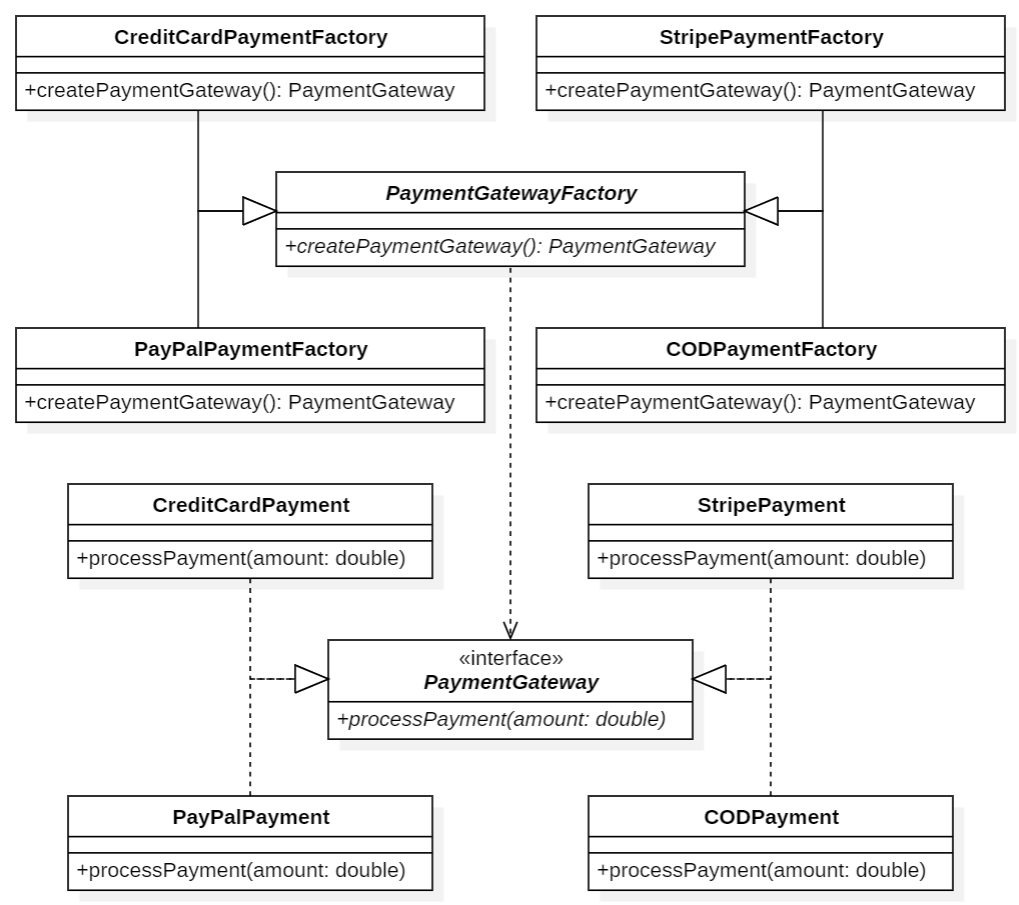
\includegraphics[width=0.9\textwidth]{../assets/screenshots/uml/factory_method.png}
        \caption{Factory Method UML Class Diagram}
    \end{figure}
\end{flushleft}

\subsubsection{Hoạt động}
\begin{flushleft}
    \begin{itemize}
        \item \textbf{Tạo đối tượng:} Khi cần tạo một đối tượng \verb|PaymentGateway| cụ thể, thay vì khởi tạo trực tiếp bằng từ khóa \verb|new|, chúng ta sẽ sử dụng một factory tương ứng. Ví dụ, để tạo một đối tượng thanh toán bằng thẻ tín dụng, ta sẽ gọi phương thức \verb|createPaymentGateway()| của \verb|CreditCardPaymentFactory|.
        \item \textbf{Đa hình:} Nhờ cơ chế đa hình, cùng một phương thức \verb|processPayment()| có thể thực hiện các hành vi khác nhau tùy thuộc vào đối tượng cụ thể được gọi. Ví dụ, khi gọi \verb|processPayment()| trên một đối tượng \verb|CreditCardPayment|, hệ thống sẽ thực hiện các logic xử lý thanh toán bằng thẻ tín dụng.
        \item \textbf{Mở rộng:} Nếu muốn thêm một phương thức thanh toán mới, ta chỉ cần tạo một lớp con mới của \verb|PaymentGateway| và một lớp factory tương ứng, không cần sửa đổi các lớp đã có.
    \end{itemize}
\end{flushleft}

\subsubsection{Khả năng ứng dụng}
\begin{flushleft}
    \begin{itemize}
        \item \textbf{Hệ thống thanh toán:} Giúp quản lý nhiều phương thức thanh toán khác nhau một cách linh hoạt.
        \item \textbf{Factory:} Tạo ra các sản phẩm khác nhau dựa trên các thông số đầu vào.
        \item \textbf{Xây dựng giao diện người dùng:} Tạo ra các đối tượng giao diện khác nhau dựa trên các cấu hình.
    \end{itemize}
\end{flushleft}

\subsubsection{Ưu nhược điểm}
\begin{flushleft}
    \begin{itemize}
        \item \textbf{Ưu điểm}
              \begin{itemize}
                  \item \textbf{Tách biệt quá trình tạo đối tượng:} Quá trình tạo đối tượng được tách biệt khỏi logic sử dụng đối tượng, giúp code rõ ràng hơn và dễ bảo trì.
                  \item \textbf{Tăng tính linh hoạt:} Dễ dàng thêm các phương thức thanh toán mới mà không ảnh hưởng đến phần còn lại của hệ thống.
                  \item \textbf{Ẩn đi các chi tiết triển khai:} Người dùng chỉ cần biết giao diện PaymentGateway, không cần quan tâm đến cách các phương thức thanh toán được thực hiện bên trong.
                  \item \textbf{Dễ kiểm thử:} Mỗi factory có thể được kiểm thử độc lập.
              \end{itemize}
        \item \textbf{Nhược điểm}
              \begin{itemize}
                  \item Mã có thể trở nên phức tạp hơn vì cần tạo thêm nhiều lớp con mới để triển khai mẫu thiết kế.
                  \item Việc có quá nhiều lớp factory có thể làm cho hệ thống trở nên khó quản lý và khó bảo trì (maintain).
              \end{itemize}
    \end{itemize}
\end{flushleft}

\subsubsection{Mã nguồn}
\codeimport{cpp}{../src/ecommerce-demo/Payment.hpp}
